\chapter{Naturalness and fine-tuning beyond the MSSM}
\label{chap:finetuning}

\chapterquote{God used beautiful mathematics in creating the world.}%
{Paul Dirac, 1902--1984}

\noindent
The null results of supersymmetry at the CMS and ATLAS collaborations have put great constraint on the masses of coloured sparticles such as the gluino and squarks, leading to 95\% C.L. exclusion limits (within certain simplifying assumptions) of about $m_{\tilde{g}} \gtrsim 1.5$ TeV for $m_{\tilde{g}} \simeq m_{\tilde{q}}$ and $m_{\tilde{g}} \gtrsim 1$ TeV for $m_{\tilde{g}} \ll m_{\tilde{q}}$ \cite{RN567,RN568,RN569,RN693,RN695}. Recent $\sqrt{s}=13$ TeV results may suggest even stronger limits, excluding up to $\sim 2$ TeV gluinos and $\sim 1.5$ TeV squarks \cite{RN697,RN698}. It is particularly these limits that have hinted at the fact that the `natural' MSSM may not be realistic. Furthermore, it has been shown that in order to keep the MSSM `natural', one must keep the sparticle masses quite below the TeV scale \cite{RN699,RN239,RN700,RN701,RN703,RN702,RN704,RN705,RN706,RN707,RN708,RN710,RN709,RN711,RN712,RN713,RN714,RN715,RN716,RN717,RN719,RN720,RN721,RN722,RN691,RN723,RN724,RN69,RN5,RN253}.
\begin{center}
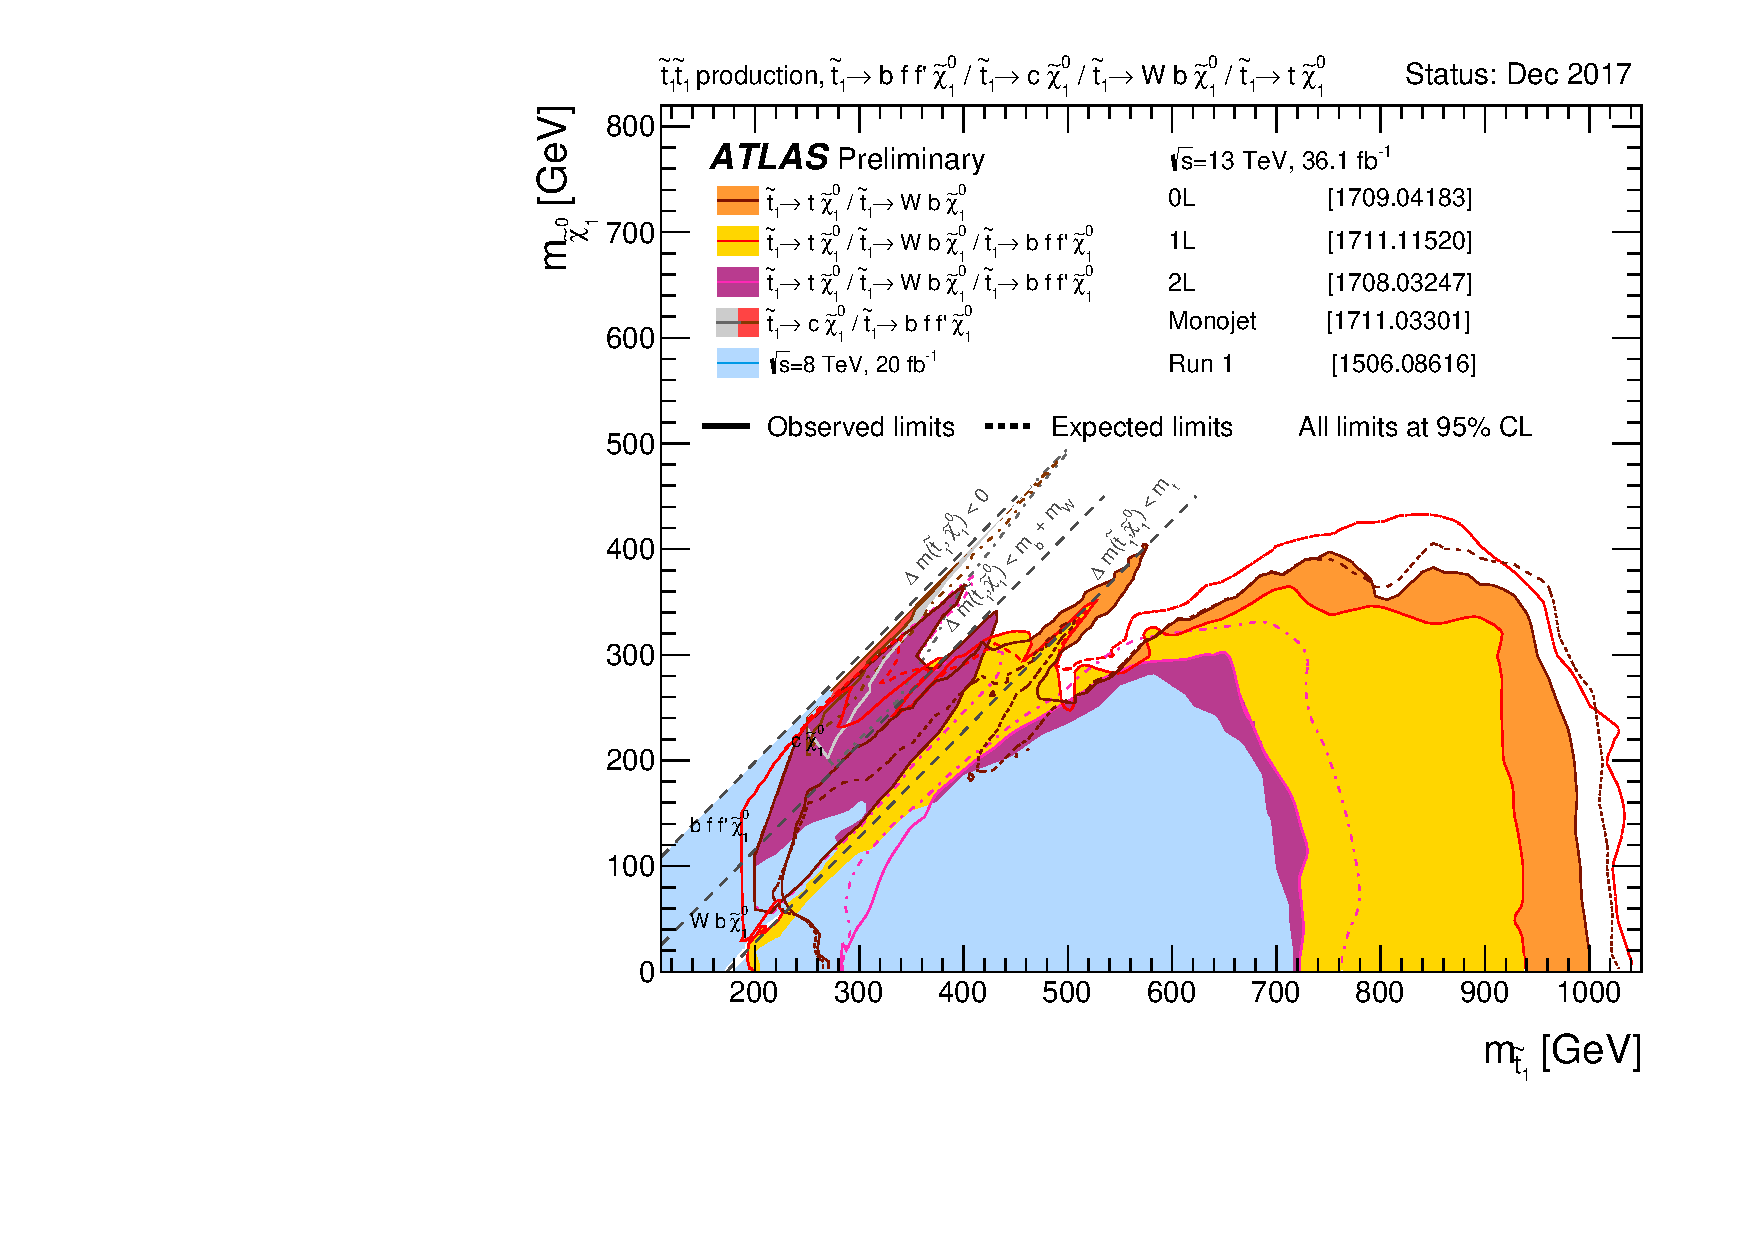
\includegraphics[scale=0.35]{figures/ATLAS_SUSY_Stop_tLSP.pdf}
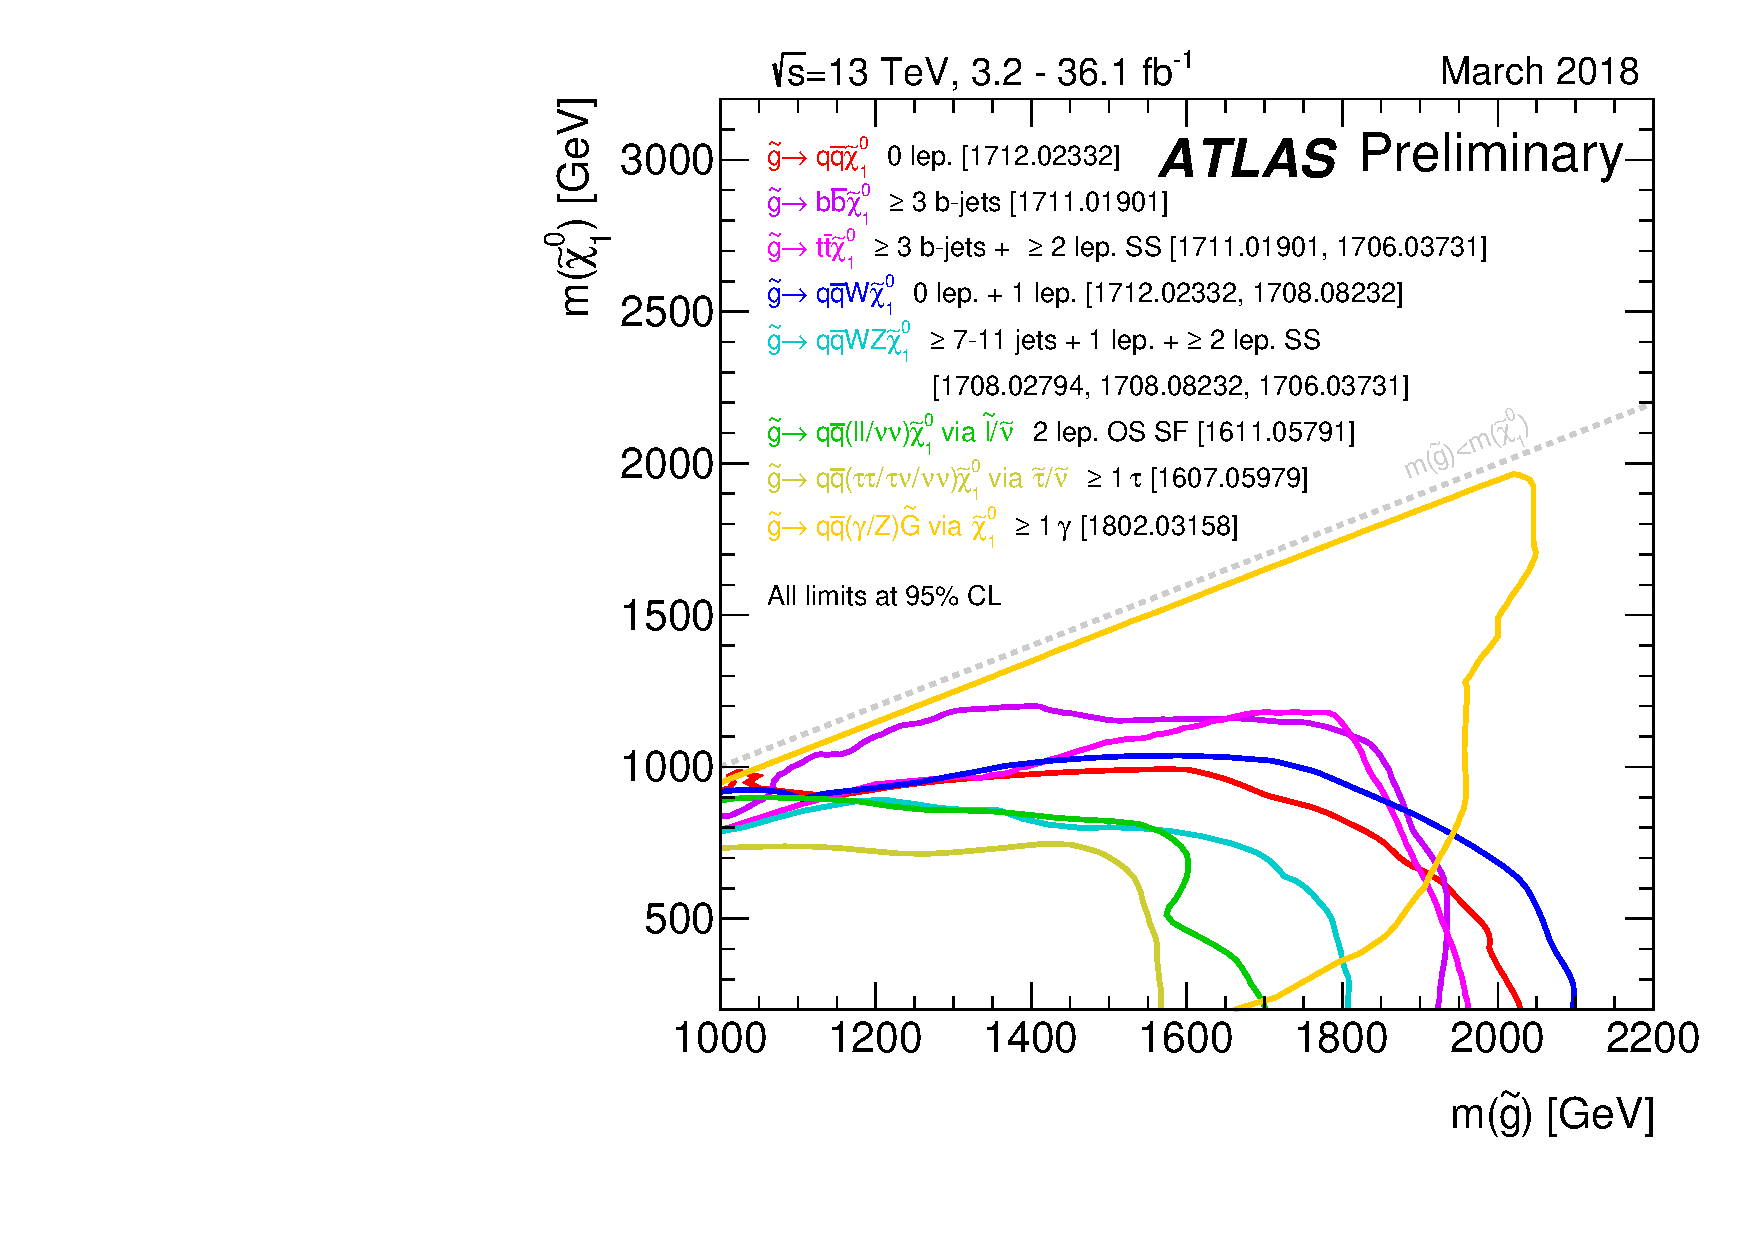
\includegraphics[scale=0.35,trim={0 0.85cm 0 0},clip]{figures/ATLAS_SUSY_Strong_all.pdf}
\captionof{figure}[Limits on stops and gluinos.]{(Left) A Summary of the dedicated searches for stop pair production from ATLAS 3.2-36 $\text{fb}^{-1}$ data at $\sqrt{s}=13$ TeV, showing the 95\% C.L. exclusion limits in the $m_{\tilde{t}_1}-m_{\tilde{\chi}^0_1}$ plane. (Right) Exclusion limits at 95\% C.L. in the $m_{\tilde{g}}-m_{\tilde{\chi}^0_1}$ plane from ATLAS $\sqrt{s}=13$ TeV data for various simplified models of gluino decaying to the lightest neutralino \cite{RN695}.}
\label{fig:SUSYlimits}
\end{center}
Many of these models at large, however, come with a number of parameter relations usually as a result from some enhanced symmetries at the high-scale. Some studies have shown that this can lead to a significant reduction in fine-tuning. For example in \cite{RN716,RN712,RN749,RN750,RN751,RN752} one finds the existence of the `gaugino focus point' corresponding to a particular hierarchy of gaugino masses at the GUT scale. This could result from the embedding of SUSY in a larger gauge group structure or even from string theory. Similarly, the low-energy spectrum may contain degeneracies in the scalar masses coming from soft SUSY breaking stemming from cancellations between the tree and loop corrections to the Higgs boson mass leading to an overall reduction in fine-tuning (the so-called `focus-point') \cite{RN90,RN704,RN753,RN754,RN755}. Although as attractive as these prospects are, we in fact have no knowledge of the UV-complete supersymmetric Standard Model, or at which energy scale this should appear. More specifically, the failure for the MSSM to remain natural seems to hint that there is physics beyond the MSSM - whatever that may be. We have already mentioned the case where certain boundary conditions at the high scale can lead to reduction in fine-tuning - however one can also consider modifications to the Renormalization Group (RG) running down to low energies.

In this section, within the framework of this effective field theory, we parameterize our ignorance of the UV-physics and consider arbitrary variation in the 20-dimensional MSSM parameter space, for differing values of the unknown new physics intermediate scales $\Lambda$ in the next section. 

 Firstly, let us consider the minimization of the tree-level MSSM potential, which gives the following condition on the mass of the $Z$-boson:
\begin{equation}
\frac{m^2_Z}{2}=\frac{m^2_{H_d}-m^2_{H_u}\tan^2\beta}{\tan^2\beta-1}-|\mu|^2 \simeq -m^2_{H_u}-|\mu|^2,
\label{eqn:mZmincond}
\end{equation}
where the far right-hand side is valid for medium-to-large values of $\tan \beta$, or when $|m_{H_d}| \lesssim |m_{H_u}|$ for $\tan \beta \gtrsim 3$. For the one-loop MSSM Coleman-Weinberg potential \cite{RN684,RN683}, one simply makes the replacements
\begin{equation}
m^2_{H_u} \rightarrow m^2_{H_u} + \Sigma^u_u, \qquad  m^2_{H_d} \rightarrow m^2_{H_d} + \Sigma^d_d,
\end{equation}
where $\Sigma^u_u$ and $\Sigma^d_d$ are the one-loop corrections which include contributions from particles and sparticles with sizable Higgs-Yukawa or gauge-Higgs couplings. Eq. \ref{eqn:mZmincond} highlights a very important feature of the MSSM. This condition intrinsically connects the SUSY breaking scale, coming from the Higgs mass terms, with the electroweak breaking scale. In fact, since the $\mu$ term sets the masses of the Higgsinos in the MSSM, natural SUSY usually requires that the Higgsinos not exceed a couple hundred GeV \cite{RN685, RN686, RN684, RN687, RN688, RN689, RN690, RN691}. As is typically the case, the soft-SUSY breaking mass for the up-type Higgs doublet, $m_{H_u}$, is usually driven to negative values at the electroweak scale, triggering EWSB.

Hence, it is clear from the last equality in Eq. \ref{eqn:mZmincond} that we must adjust the low-energy values of $m_{H_u}$ and $\mu$ in such a way to reproduce $m_Z \simeq 91$ GeV. This can be achieved in a `natural' way when these adjustments are not sensitive to the variation in the fundamental parameters of the theory defined at some high scale, $\Lambda$. Quantitatively measuring this sensitivity, we invoke the standard Barbieri-Guidice measure \cite{RN239}:
\begin{equation}
\Delta = \max \left\{\left| \frac{a_i}{m^2_Z}\frac{\partial m^2_Z}{\partial a_i} \right| \right \},
\label{eqn:BGmeasure}
\end{equation}
where the $a_i$ are the fundamental parameters of the low-energy effective MSSM theory. These are of course renormalized through the RGEs down to the SUSY scale $M_{SUSY}$ at which the fine-tuning is actually evaluated. The quantity $\Delta$ represents the degree to which one must tune the independent parameters to correctly reproduce the electroweak scale. The application of the measure in the curly brackets in Eq. \ref{eqn:BGmeasure} to the right-hand side of Eq. \ref{eqn:mZmincond} results in
\begin{equation}
\frac{a_i}{m^2_Z}\frac{\partial m^2_Z}{\partial a_i}=\frac{2 a^2_i}{m^2_Z}\left( -\frac{\partial \mu^2}{\partial a^2_i} -\frac{\partial m^2_{H_u}}{\partial a^2_i} \right).
\end{equation}
Naively, one can estimate this fine-tuning at tree-level from $a_i=\{\mu^2,m^2_{H_u}\}$. We find
\begin{equation}
\Delta_{\mu} = -\frac{2\mu^2}{m^2_Z},\qquad \Delta_{m^2_{H_u}} = -\frac{2 m^2_{H_u}}{m^2_Z}.
\end{equation}
Again this tree-level analysis shows that in order to achieve low fine-tuning, one must have the absolute values of $\mu$ and $m^2_{H_u}$ at the electroweak scale to be comparable to the mass of the $Z$-boson.

Another question we may ask is: how much fine-tuning is actually acceptable? Of course this may differ among phenomenologists, however it is reasonable to accept that a value of $\Delta$ greater than 100 ($\Delta^{-1} \sim 1\%$ - corresponding to cancellations no more than 2 orders of magnitude) would amount to a fine-tuned theory. 

We approach the problem of fine-tuning in two ways. Firstly, we assume that the UV physics beyond the MSSM enters at a low enough scale such that the RG running of the ``fundamental" parameters is not strong enough to destabilize the electroweak minimum relationship in Eq. \ref{eqn:mZmincond}. Secondly, we look for relationships among parameters in the RGEs that correspond to infrared fixed-point behavior - implying that the values of the parameters satisfying the electroweak minimum condition are not particularly sensitive to their values at the input scale. We explore this case in sections \ref{sec:QFPMSSM} and \ref{sec:QFPscan}.

\section{General MSSM parameter scan}
\label{sec:generalscan}

Here we present our results for a general parameter scan over the 20-dimensional MSSM parameter space. We take a random sampling of the following parameter ranges:
\begin{eqnarray}
-3000\,\text{GeV} <& M_1,M_2 &< 3000\,\text{GeV}, \nonumber \\
&M_3 &< 3000\,\text{GeV}, \nonumber \\
-(3000)^2\,\text{GeV}^2 <& m^2_{H_u},m^2_{H_d} &< (3000)^2\,\text{GeV}^2, \nonumber \\
& m^2_{i_{1,2}} &< (3000)^2\,\text{GeV}^2, \nonumber \\
& m^2_{i_3} &< (3000)^2\,\text{GeV}^2, \nonumber \\
-3000\,\text{GeV} <& A_t,A_b,A_{\tau} &< 3000\,\text{GeV}, \nonumber \\
1 <& \tan \beta &< 50, \nonumber \\
&sign(\mu)&=\pm 1.
\label{eqn:param2}
\end{eqnarray}
where $i=(Q,\bar{u},\bar{d},L,\bar{e})$. Note that the first and second generation scalar soft masses are taken to be degenerate and similarly we assume no flavour mixing at the input scale (i.e. these are the diagonal entries of the matrices, we assume the off-diagonal entries are zero). In contrast to the philosophy adopted in chapter \ref{chap:muong-2}, and in virtue of the discussion in the previous section, we obviously cannot invoke decoupling of the third-generation squarks or gluino which are the main culprits in MSSM fine-tuning. However, the subsequent results in this chapter suggest that such a heavy spectra in the order of a few TeVs may indeed still remain natural pertaining to the important boundary conditions that we specify.

Eqs. \ref{eqn:param2} are the fundamental parameters of the theory entered at the following representative values of $\Lambda$:
\begin{equation}
\Lambda \in \left[10^5,10^{10},10^{16} \right]\,\text{GeV}.
\end{equation}
We employ the full two-loop RGEs using \texttt{SPHENO-3.3.8} \cite{RN178} combined with \texttt{SARAH} \cite{RN310} to compute both the MSSM spectrum and the fine-tuning measure. The parameters included in the calculation of the fine-tuning measure in Eq. \ref{eqn:BGmeasure} are the gaugino masses $M_1,M_2,M_3$, Higgs soft-breaking masses $m^2_{H_u},m^2_{H_d}$, 3rd generation scalar masses $m^2_{Q_3},m^2_{\bar{u}_3},m^2_{\bar{d}_3},m^2_{L_3},m^2_{\bar{e}_3}$, the trilinear couplings $A_t,A_b,A_{\tau}$, and the terms $\mu$ and $B_{\mu}$, all computed at the corresponding scale $\Lambda$. The top (pole) mass is set to 173 GeV. We also compute the DM relic density $\Omega_{DM} h^2$ and spin-independent WIMP-nucleon cross-section assuming a neutralino DM candidate using \texttt{micrOmegas-4.3.2} \cite{RN621}.

Points which have a vacuum in the electroweak broken phase are chosen which also satisfy $\Delta \leq 1000$ are subsequently passed through the following constraints:
\begin{itemize}
	\item Direct searches for the slepton and chargino at LEP produce the mass limits on the first two generation sleptons and lightest chargino \cite{RN493}:
	\begin{eqnarray}
	m_{\widetilde{l}_L},m_{\widetilde{l}_R} &>& 100\,\text{GeV}, \qquad (l=e,\mu), \\
	m_{\widetilde{\chi}^{\pm}_1} &>& 105\,\text{GeV},
	\end{eqnarray}
    \item We require the lightest Higgs boson mass in the range $122 < m_h < 128\,\text{GeV}$ \cite{RN62,RN63},
    \item We require the lightest neutralino $\widetilde{\chi}^0_1$ as the LSP and $m_{\widetilde{\chi}_1^0}>30\,\text{GeV}$ to be consistent with the bound on light MSSM neutralino dark matter \cite{RN232,RN775},
    \item We satisfy the 3 sigma upper bound on dark matter relic density observed by the Planck collaboration given by $\Omega_{Planck}h^2 = 0.112 \pm 0.006$ \cite{RN498}. For points with underabundant dark matter, we assume there may be some additional contribution from non-thermal candidates, such as the axion.
    \item We use the recent data from XENON1T \cite{RN606} to constrain the points with results from direct detection experiments, where we rescale the spin-independent cross-section $\sigma^{SI}$ to the observed relic density by $(\Omega_{DM} h^2/\Omega_{Planck}h^2)$,
    \item We check the bounds from Higgs searches at LEP, Tevatron and LHC implemented using \texttt{HiggsBounds-4.3.1} \cite{RN170},
    \item We also check important $B$-physics and flavour constraints, namely $\mathcal{B}(B\rightarrow X_s\gamma)$ and $\mathcal{B}(B_{S} \rightarrow \mu^{+}\mu^{-})$. The measured values we use are $\mathcal{B}(B\rightarrow X_s\gamma)_{\text{exp}}=(3.55 \pm 0.26)\times10^{-4}$ \cite{RN773} and the upper bound $\mathcal{B}(B_{S} \rightarrow \mu^{+}\mu^{-})_{\text{exp}}<1.08\times10^{-8}$ (95$\%$ CL) \cite{RN772}. These are calculated using \texttt{FlavorKit} \cite{RN771} as part of the \texttt{SPheno}/ \texttt{SARAH} package. Where an upper and lower bound are shown, we constrain our points to within $3\sigma$ of the quoted value.
\end{itemize}
We do not impose constraints from direct gluino/stop-squark searches from LHC as the limits are largely model-dependent and would require a dedicated recasting. Besides, there are many cases in which the spectrum may be compressed to easily avoid these LHC search constraints. In Figure \ref{fig:generalfine} we show the dependence on the fine-tuning measure on the gluino mass $M_{\tilde{g}}$ and lighter stop mass $M_{\tilde{t}_1}$.

\begin{center}
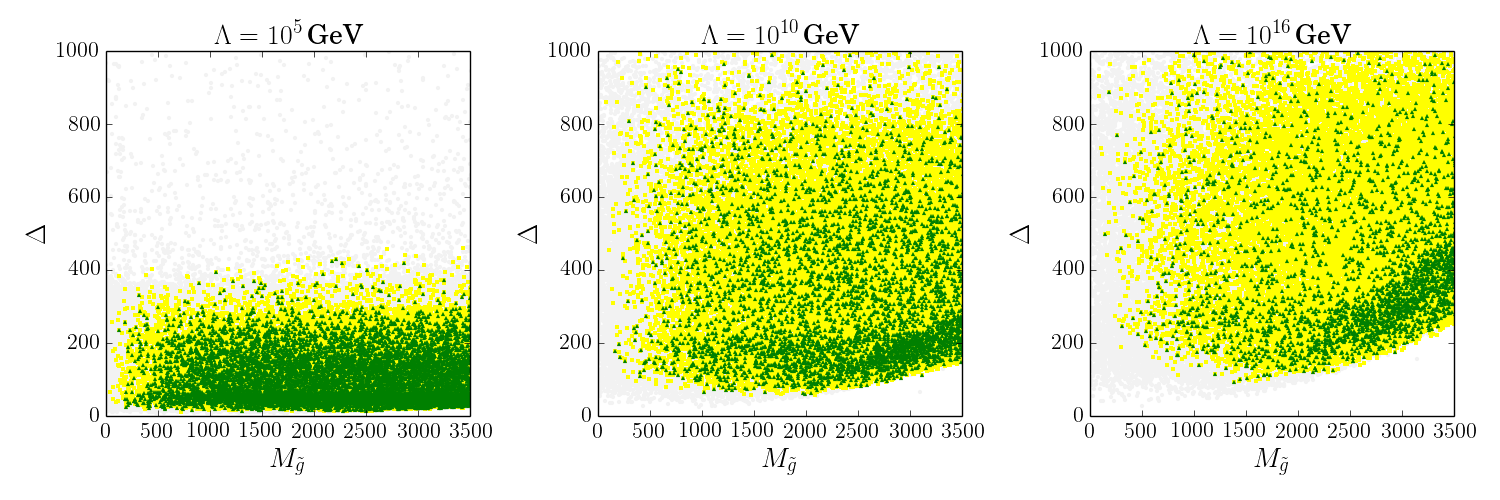
\includegraphics[scale=0.4]{figures/plot_mglu.png}
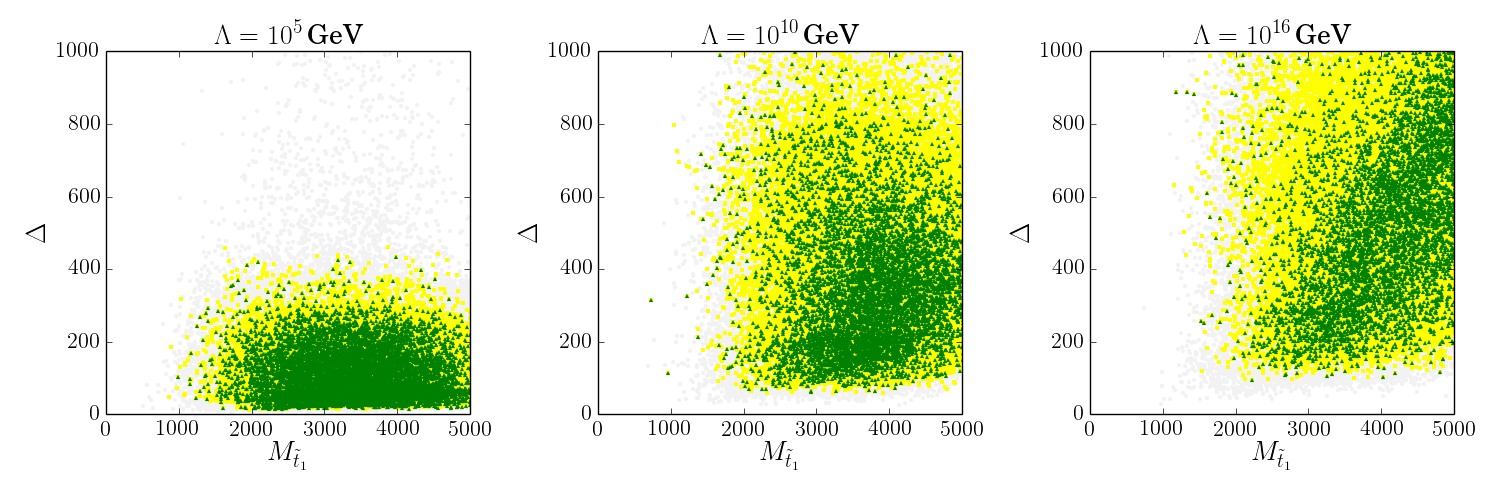
\includegraphics[scale=0.4]{figures/plot_mt1.png}
\captionof{figure}[Fine-tuning measure.]{Fine-tuning measure as a function of the gluino mass (top panel) and lighter stop mass (bottom panel) for three representative \acrshort{np} scales. Yellow squares contain LEP and Higgs mass constraints as well as $B$-Physics and Higgs precision constraints. The green squares are a subset of these containing DM relic density and direct detection constraints.}
\label{fig:generalfine}
\end{center}

Reductions in fine-tuning for the lower scales are indeed proportional to the amount of renormalization `running time', $\log \Lambda^2/m^2_Z$, and hence we see one can achieve a fine-tuning measure around $\mathcal{O}(10)$ for $\Lambda=100$ TeV. Furthermore, as we see in the plots in Figure \ref{fig:DMfine}, the dark matter constraints are satisfied relatively easily.

Since the electroweakino masses $M_1$ and $M_2$ enter the RGE for the up-type Higgs soft-breaking mass rather mildly (proportional to their respective gauge couplings), models with underabundant dark matter that are still compatible with direct detection constraints can exist without a strong contribution to the fine-tuning.

\begin{center}
	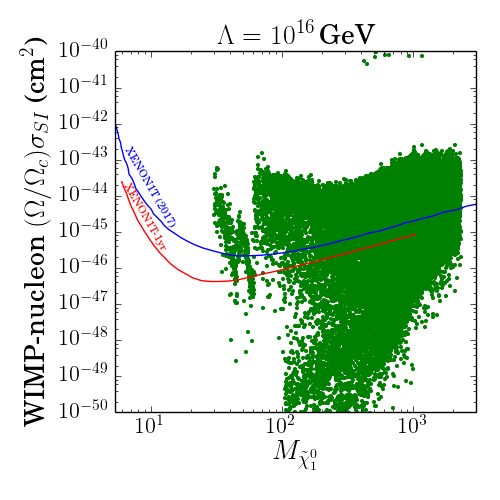
\includegraphics[height=0.21\paperheight]{figures/plot_nucleon.png}
	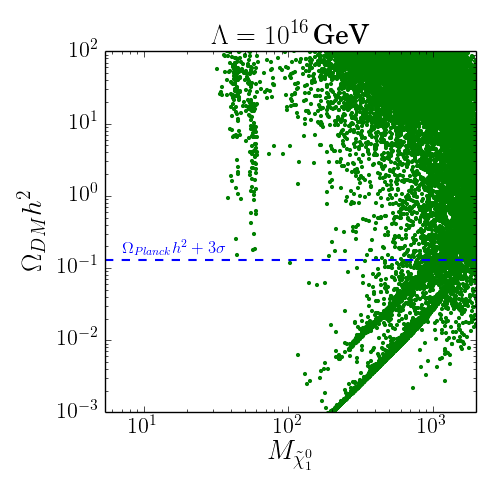
\includegraphics[height=0.21\paperheight]{figures/plot_relic.png}
	\captionof{figure}[Relic density and WIMP-nucleon spin-independent cross-section.]{Left: Relic density $\Omega_{DM}$ as a function of the LSP mass corresponding to the red squares in the rightmost panels of Figure \ref{fig:generalfine}. The dotted line corresponds to the PLANCK measurement of $\Omega_{Planck}h^2 = 0.112 \pm 0.006$ \cite{RN498}. Right: WIMP-nucleon spin-independent cross-section as a function of the LSP mass for the points shown in the left panel. Since we allow the LSP to be underabundant after freeze-out, we rescale the cross-section by the factor $\Omega/\Omega_{c}$ where $\Omega_{c}$ corresponds to the measured Planck Collaboration value. The solid lines corresponds to the XENON1T 2017 \cite{RN606} and the recent 1 tonne $\times$ year \cite{RN770} results. Similar plots exist for $\Lambda=10^{5}$ and $10^{10}$ GeV.}
	\label{fig:DMfine}
\end{center}

\section{The top-Yukawa infrared quasi fixed-point in the MSSM}
\label{sec:topqfp}

Consider the RGEs for the strong gauge coupling $g_3$ and the top-Yukawa coupling $y_t$ (given in appendix \ref{app:onelooprge}), in the absence of 2-loop or electroweak effects,
\begin{eqnarray}
\frac{dg_3}{dt}&=&-\frac{3g^2_3}{16\pi^2}, \\
\frac{dy_t}{dt}&=&\frac{y_t}{16\pi^2}\left( 6y^2_t - \frac{16}{3}g^2_3 \right),
\end{eqnarray}
where $t=\log (Q/Q_0)$ and $Q$ is the energy scale. One can easily verify that the ratio
\begin{equation}
\left(\frac{y^2_t}{g^2_3}\right)^{FP}=\frac{7}{18},
\end{equation}
is renormalization-invariant. This is the \textit{quasi-infrared fixed-point} (\acrshort{qfp}) \cite{RN747,RN748}, also known as the Pendleton-Ross fixed-point, since the top Yukawa coupling will track closer to the strong gauge coupling as one continues into the infrared. We show this behavior in Figure \ref{fig:topyuk}.

\begin{center}
\includegraphics[width=0.7\linewidth]{figures/TopYuk.png}
\captionof{figure}[Top-Yukawa quasi fixed-point behavior.]{The top Yukawa coupling $y_t$ expresses a quasi-infrared fixed-point evolving from $\Lambda=M_{GUT}$ to $m_Z$ at two-loop renormalization. Taken from \cite{RN746}.}
\label{fig:topyuk}
\end{center}

If one starts with a large top Yukawa coupling at a high scale, $\Lambda$ (could be the \acrshort{gut} scale), then we can even compute the value of $\tan \beta$ from the running top mass:
\begin{equation}
m_t(m_t)=\frac{y^{FP}_t v}{\sqrt{2}} \sin \beta,
\end{equation}
which of course is distinguishable from the physical top mass $m^{\text{pole}}_t$ which receives sizable one-loop corrections from (i) QCD gluons in the SM\footnote{This has the well-known result in the $\overline{DR}$ renormalization scheme \cite{RN741}:
\begin{equation}
\left(\frac{\Delta m_t}{m_t}\right)_{QCD}=\frac{5g^2_3}{12 \pi^2}.
\end{equation}}
and (ii) stops/gluinos from SUSY
\begin{equation}
m_t (m_t)= \frac{m^{\text{pole}}_t}{1 + \left(\frac{\Delta m_t}{m_t}\right)_{QCD} + \left(\frac{\Delta m_t}{m_t}\right)_{SUSY}},
\end{equation}
where the SUSY corrections are given by \cite{RN741,RN742,RN743,RN744,RN745}
\begin{eqnarray}
\left(\frac{\Delta m_t}{m_t}\right)_{SUSY}=-\frac{g^2_3}{12 \pi^2} \left\{ B_1 (m_t,m_{\tilde{g}},m_{\tilde{t}_1}) +B_1 (m_t,m_{\tilde{g}},m_{\tilde{t}_2}) \right. \\
\left. -\sin(2\theta_t)\frac{m_{\tilde{g}}}{m_t}\left[ B_0 (m_t,m_{\tilde{g}},m_{\tilde{t}_1}) -B_0 (m_t,m_{\tilde{g}},m_{\tilde{t}_2})\right] \right\},
\end{eqnarray}
where $\theta_t$ is the stop mixing angle and
\begin{equation}
B_n (p;m_1,m_2)=-\int^1_0 dx x^n \log \left[ \frac{(1-x)m^2_1+xm^2_2-x(1-x)p^2}{m^2_t}\right].
\end{equation}
Using the observed value for the top pole mass, this predicts a value for $\tan \beta$ of about 1.5 \cite{RN740}, which produces too light a Higgs boson mass at least at tree-level, requiring large stop-loop corrections (and/or stop mixing).

\section{Other QFPs in the MSSM and fine-tuning}
\label{sec:QFPMSSM}

Since the fixed-point property of $y_t$ has been well-known for a while, some studies have focused on the existence of quasi-fixed points for other couplings in the MSSM, such as the soft SUSY-breaking parameters when $y_t$ is in its quasi-fixed regime \cite{RN285,RN255,RN256,RN249,RN250,RN251}. In fact, it has been found that many of the soft SUSY-breaking masses have low-energy predictions independent of their high-scale input.

Our goal is to study the implications of these QFPs on the fine-tuning measure in the MSSM. In particular, because of the insensitivity of some of the low-energy parameters to their values at the high-scale, we would expect the fine-tuning measure to be significantly reduced in regions of QFP attraction.

Firstly, consider the one-loop RGE for the superpotential $\mu$ term
\begin{equation}
\frac{d}{dt}\mu=\frac{\mu}{16\pi^2}\left[3y^*_ty_t+3y^*_by_b+y^*_{\tau}y_{\tau}-3g^2_2-\frac{3}{5}g^2_1\right].
\end{equation}
where $t=\log(\Lambda^2/Q^2)$, where $Q$ is an arbitrary renormalization scale. Evidently, $\mu=0$ is a fixed-point of the theory, and moreover if $\mu$ is taken small at $\Lambda$ (say $\mu \sim m_Z$) then it shall stay small running to low energies (to all orders in perturbation theory). The evolution of $m^2_{H_u}$ with the energy scale is a little more involved, due to couplings to heavier particles in the spectrum:
\begin{equation}
\frac{d}{dt}m^2_{H_u}=\frac{1}{16\pi^2}\left[3X_t-6g^2_2|M_2|^2-\frac{6}{5}g^2_1|M_1|^2+\frac{3}{5}g^2_1S\right],
\label{eqn:mHubeta}
\end{equation}
where
\begin{equation}
S\equiv m^2_{H_u}-m^2_{H_d}+\text{Tr}[m^2_Q-m^2_L-2m^2_{\bar{u}}+m^2_{\bar{d}}+m^2_{\bar{e}}],
\end{equation}
and
\begin{equation}
X_t=2|y_t|^2(m^2_{H_u}+m^2_{Q_3}+m^2_{\bar{u}_3}+|A_t|^2).
\end{equation}
Since we know that $y_t$ is quasi-fixed in the infrared, a large $y_t$ at the high-scale enhances the initial contribution from $X_t$ at $\Lambda$, especially if $m^2_{H_u}$ is initially large. Similarly, if $M_1$ and $M_2$ are initially small, the remaining terms in Eq. \ref{eqn:mHubeta} are subdominant (they are also naturally suppressed by the square of the electroweak gauge couplings). We can write the RGE for $m^2_{H_u}$ in an approximate form:
\begin{equation}
\frac{d}{dt}m^2_{H_u}=\frac{6 y^2_t}{16\pi^2}m^2_{H_u}.
\label{eqn:mHubeta2}
\end{equation}
Similar to the $\mu$ parameter, this expresses a fixed point for $m^2_{H_u}=0$. From the observation in Eq. \ref{eqn:mHubeta2}, there is another important fixed-point we can see by defining the sum:
\begin{equation}
\Sigma=m^2_{H_u}+m^2_{Q_3}+m^2_{\bar{u}_3}+|A_t|^2,
\end{equation}
from which the beta function for $\Sigma$ satisfies:
\begin{equation}
\frac{d}{dt}\Sigma=\frac{3 y^2_t}{4\pi^2} \Sigma - \frac{2}{\pi^2}g_3^2 M^2_3.
\end{equation}
This clearly has a fixed point $\Sigma=0$ in the limit $M_3 \rightarrow 0$. However, due to the dynamics of $g_3$ and $M_3$, which increase in the infrared, we would expect a significant positive contribution to the evolution of $\Sigma$. In fact, this is evidence for the large fine-tuning present in a heavier spectrum. One finds for a positive $\Sigma$ at the weak scale, one must have a large (and negative) $m^2_{H_u}$ to cancel the 3rd generation squark masses $m^2_{Q_3}$ and $m^2_{\bar{u}_3}$. Similarly, since these parameters increase significantly in the infrared with large $y_t$, they can tend to destabilize $m^2_{H_u}$ very quickly. For this reason, we also consider the case of negative stop mass-squared values at the input scale\footnote{Negative stop mass-squared at the GUT scale, for example, can lead to a potential with a D-flat direction that is unbounded from below. This is improved with large loop corrections but can generate a large charge-colour breaking minimum which can be tunneled to by the EW minimum (if it has lower potential energy) \cite{RN778}. For the tunneling rate to be longer than the age of the universe (metastable), this leads to the following constraint on the running masses, $m_{\tilde{t}}(m_Z) \gtrsim \frac{1}{10}M_3 (m_Z)$ \cite{RN769}. This is easily satisfied in our scan.}. These have been studied previously in some gauge messenger models \cite{RN776} and also in the MSSM \cite{RN769,RN777} at the GUT scale. We show the evolution of $\Sigma$ and these soft-breaking masses in Figure \ref{fig:rgeplots}.

\section{Parameter scan in the quasi-fixed point region}
\label{sec:QFPscan}

In the following section we choose a large input top Yukawa coupling, $1 < y_t \lesssim \sqrt{4\pi}$, to enhance the running of $m^2_{H_u}$. This also requires the dominance of $m^2_{H_u}$ over the other scalar mass-squared parameters, most notably $m^2_{Q_3}$ and $m^2_{\bar{u}_3}$ individually. These will also tend to grow significantly with large $y_t$ into the infrared. Furthermore, the up-type Higgs soft-breaking mass parameter is also initially chosen to be large and negative, which is driven to small negative values at the weak scale, exploiting the quasi-fixed point behavior.

This scenario differs from the well-studied Radiative Electroweak Symmetry Breaking (\acrshort{rwesb}) mechanism \cite{RN563,RN903,RN904,RN905,RN907}, described as early as the 1980's, where the renormalization group equations drive $m^2_{H_u}$ to negative values at the weak scale, triggering electroweak symmetry breaking. An extraordinary property of this behavior is that the squarks and sleptons physical mass-squared can still remain positive. However, we also allow the stop masses to be tachyonic at the input scale, where their physical mass-squared values are driven positive at the weak scale. Although REWSB has the interesting property of naturally connecting electroweak symmetry breaking with SUSY breaking, we focus on a more unique set of boundary conditions in this framework. More precisely, we scan over the following modified parameter space:
\begin{center}
	\includegraphics[width=0.45\textwidth]{figures/sum100.png}
	\includegraphics[width=0.45\textwidth]{figures/rge100.png}
	\includegraphics[width=0.45\textwidth]{figures/sum1000.png}
	\includegraphics[width=0.45\textwidth]{figures/rge1000.png}
	\captionof{figure}[Quasi fixed-point behavior of the parameter $\Sigma$.]{Evolution of the parameter $\Sigma$ to the infrared fixed-point and soft mass parameters input at $\Lambda=10^{16}$ GeV with $m^2_{Q_3}=m^2_{\bar{u}_3}=-10^5\,\text{GeV}^2$, $A_t=-100$ GeV and $\tan \beta=10$. The three separate curves are shown for different initial values of: Top Row: $M_3=100\,\text{GeV},m^2_{H_u}=-10^5, -5\times 10^5, -10^6\, \text{GeV}^2$. Bottom Row: $M_3=1000\,\text{GeV},m^2_{H_u}=-5\times10^4, -10^5, -5\times10^5\, \text{GeV}^2$.}
	\label{fig:rgeplots}
\end{center}
\begin{eqnarray}
-3000\,\text{GeV} <& M_1,M_2 &< 3000\,\text{GeV}, \nonumber \\
&M_3 &< 3000\,\text{GeV}, \nonumber \\
-(3000)^2\,\text{GeV}^2 <& m^2_{H_u} &< 0, \nonumber \\
0 <& m^2_{H_d} &< (3000)^2\,\text{GeV}^2, \nonumber \\
0<& m^2_{i_{1,2}} &< (3000)^2 \,\text{GeV}^2, \nonumber \\
0<& m^2_{L_{3},\bar{e}_{3},\bar{d}_{3}} &< (3000)^2 \,\text{GeV}^2, \nonumber \\
-(1000)^2 \,\text{GeV}^2 <& m^2_{Q_{3},\bar{u}_{3}} &< (1000)^2 \,\text{GeV}^2, \nonumber \\
-3000\,\text{GeV} <& A_t,A_b,A_{\tau} &< 3000\,\text{GeV}, \nonumber \\
1 <& \tan \beta &< 50, \nonumber \\
&sign(\mu)&=\pm 1, \nonumber\\
1 <& y_t &< 3.
\end{eqnarray}
We also choose three representative high scales to enhance the running of $m^2_{H_u}$ through the top Yukawa coupling:
\begin{equation}
\Lambda \in \left[10^{10},10^{16},10^{19} \right]\,\text{GeV}.
\end{equation}
Again, satisfying the constraints detailed in section \ref{sec:generalscan}, we show the plots corresponding to the quasi-fixed point behavior in Figure \ref{fig:QFPplots}.
\begin{center}
	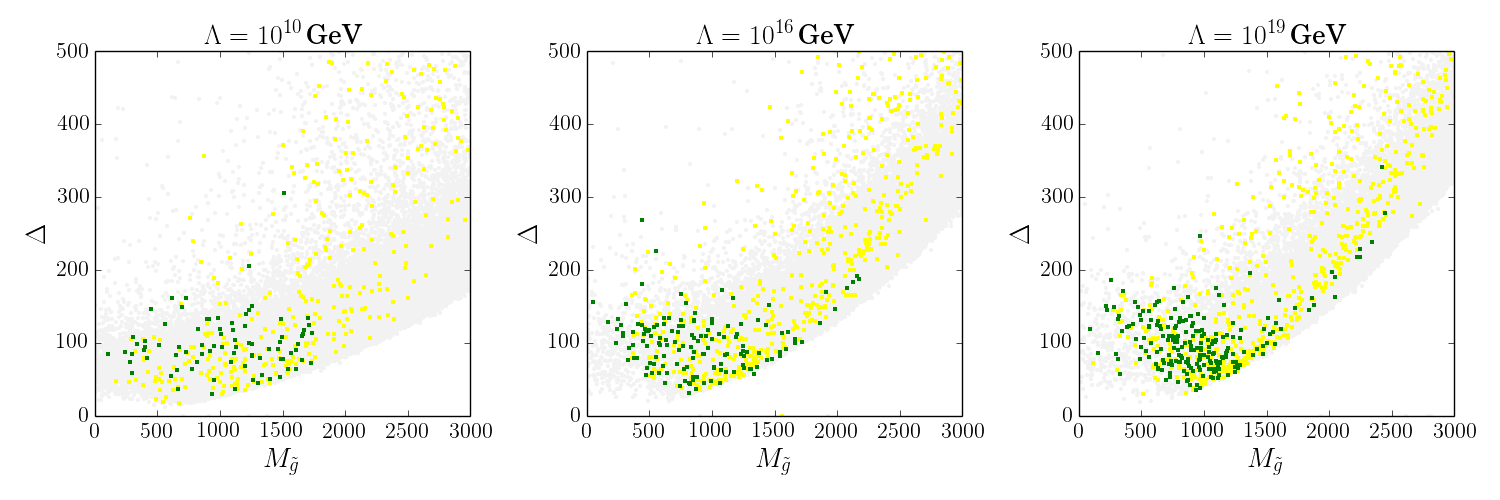
\includegraphics[scale=0.4]{figures/plot_mglu_QFP.png}
	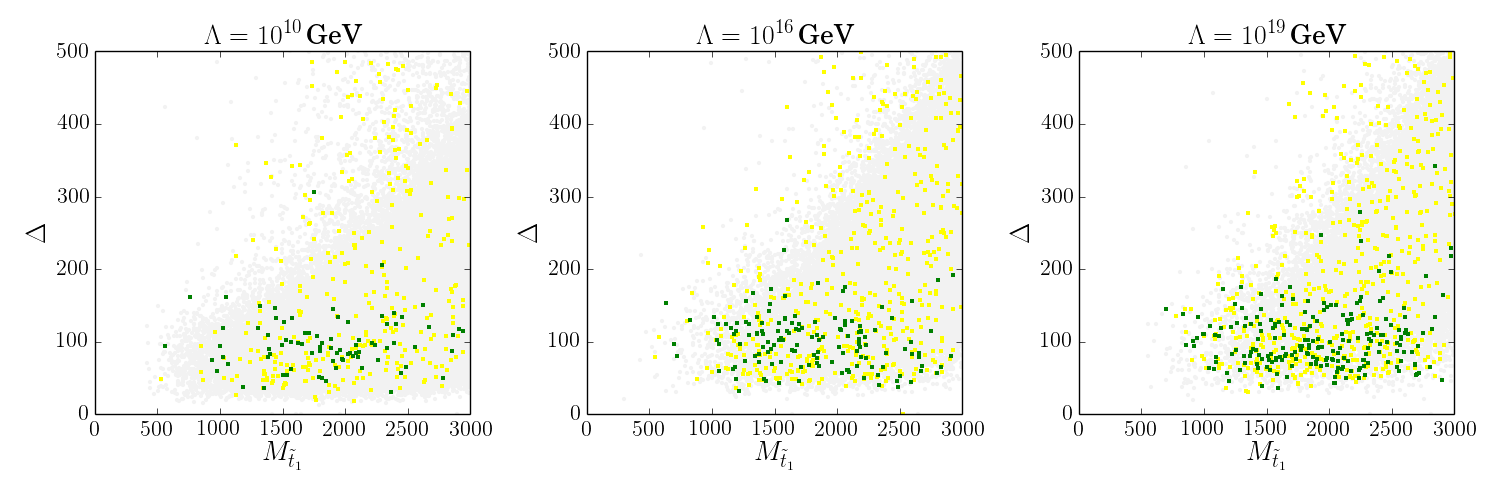
\includegraphics[scale=0.4]{figures/plot_mt1_QFP.png}
\captionof{figure}[Fine-tuning measure in the quasi-fixed point regime.]{Same as in Figure \ref{fig:generalfine} with higher $\Lambda$ scales and in a narrower scan range supporting the infrared fixed-point behavior for $\Sigma$. Note the smaller y-axis range. Small fine tuning of $\Delta < O(100)$ can be achieved even for heavier sparticle masses $> 1$ TeV.}
\label{fig:QFPplots}
\end{center}
The plots shown in Figure \ref{fig:QFPplots} confirm our expectation showing significant reduction in fine-tuning in the quasi-fixed point regime, even holding at very high NP scales.

\section{Concluding remarks}

Through our consideration of naturalness, and in light of current experimental limits from the LHC, we believe that this is hinting towards evidence for physics beyond the MSSM. In this way, the MSSM is treated as an effective theory all the way up to a scale $\Lambda$ with no a priori assumption on the origin of soft-breaking terms. This is alternative to the often used boundary conditions assuming common scalar or gauginos at the GUT scale, for example. For our definition for acceptable fine-tuning, we observe the comfortable accommodation of multi-TeV coloured sparticles when the scale of new physics is even as low as $\Lambda = 10^{10}$ GeV and most certainly for $\Lambda = 100$ TeV. More precisely, we see the reduction of fine tuning from $\Delta \sim \mathcal{O}(100)$ for $\Lambda = 10^{16}$ GeV to $\Delta \sim \mathcal{O}(10)$ for $\Lambda = 10^5$ GeV in this case. But perhaps of greater interest is the existence of low-fine tuning ($\Delta < \mathcal{O}(100)$) when the MSSM behaves close to a quasi-fixed regime where the dynamics of the soft-breaking parameter $m^2_{H_u}$ becomes less sensitive to its value at $\Lambda$. Because of the importance of the gluino mass $M_3$ in the evolution of $m^2_{H_u}$ to low-energies, we find an upper limit of about $\sim$1.5 TeV on the gluino satisfying this naturalness criteria (and all other relevant constraints) when input at around the GUT scale and above. These results are of course indicative only - one could always perform a dedicated collider recasting outside the scope of our study. Nonetheless, this calls for a further exploration into non-standard UV completions to the MSSM.

